\chapter{Introduction}
\label{c:intro}


% Unlike western languages such as English, which utilize keybaord devices that map directly to the letters of their words, Chinese characters consist of at least tens of thousands of characters that cannot be trivially mapped into computing keyboard devices. One form of input that hardware designers have chosen is to alternatively capture existing Latin-based romanization systems that can rely on existing computing keyboard devices to similarly type Chinese characters. Such mechanisms have greatly enabled many users of native Chinese language users to perform many computing tasks analogously to their western counterparts ranging from typing documents, browsing the web, and communicate with others in social media, which eventually led to the Chinese language being one of the most popular languages utilized on the internet.

As miniaturization and battery technology improve, major electronics manufacturers have created smartwatches, which contain the processing power and memory of a computer or a smartphone and feature 4G connectivity, GPS, accelerometers, heart beat sensors and so on. These smartwatches can provide interactions with the digital world without one having to carry a phone, for example when doing outdoor sports.

Even though smartwatch devices have become more and more comparable to smartphones in terms of computing power, user interaction can be tricky due to the limited screen size and small form factor. Voice input, while reliable and fast in most cases, is not always socially acceptable and may not be a viable option in noisy environments or when entering out-of-vocabulary text such as addresses or passwords. As such, easy-to-use and accurate text input methods are an important aspect of smartwatch devices, and platform developers such as Google now include touch-based text input methods by default and allow users to add 3rd party input methods.

% ONE SUGGESTION: possibly mention that existing input techniques that still assume conventional QWERTY keyboard assumptions do not consider the smaller form factors and constrained screen sizes found in the newer contributions and growing ubiquity of smartwatches (e.g., not optimize, come up with something more appropriate)

In this paper, we design and implement 3 fully functional Chinese soft keyboards for modern circular smartwatches. We propose an adaptive quasi-QWERTY keyboard that enlarges the next possible keys to improve speed and accuracy, an adaptive 2-stage keyboard that allows any Pinyin syllable to be entered with a fixed number of 2 key presses, and a standard QWERTY keyboard with 26 keys optimized for the small screen size. All 3 keyboard implementations use the same Pinyin-to-Chinese-Character conversion engine to allow for a fair comparison in our user study.

\begin{figure}
  \centering
  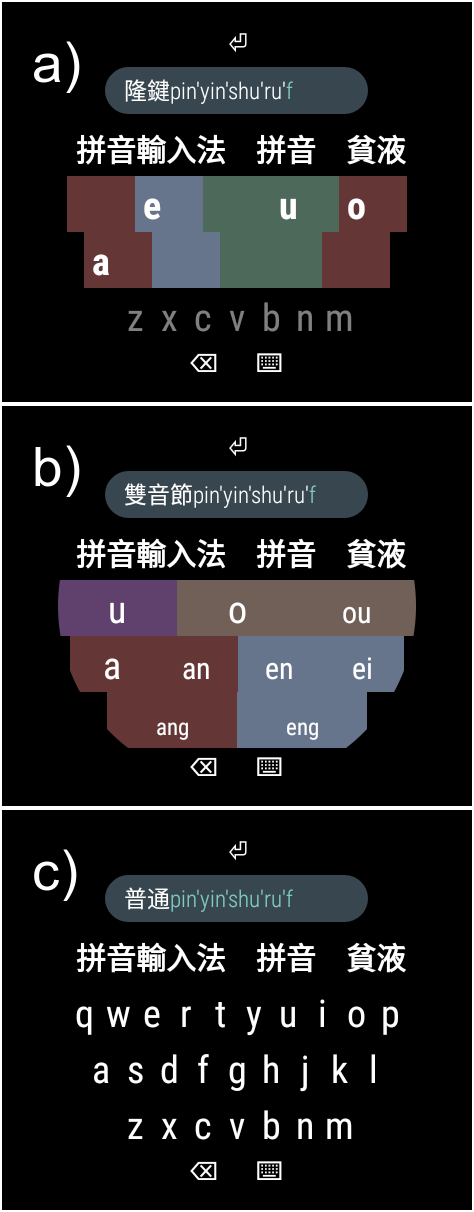
\includegraphics[width=\textwidth,height=0.9\textheight,keepaspectratio]{figures/stripe_banner_layouts}
  \caption{Keyboards for Chinese text input on smartwatches used in our study: (a) Growing Finals, (b) Pinyin Syllables and (c) Standard QWERTY.}~\label{fig:figure1}
\end{figure}
